% Options for packages loaded elsewhere
\PassOptionsToPackage{unicode}{hyperref}
\PassOptionsToPackage{hyphens}{url}
%
\documentclass[
  10pt,
  letterpaper,
  DIV=11,
  numbers=noendperiod,
  twoside]{scrartcl}

\usepackage{amsmath,amssymb}
\usepackage{setspace}
\usepackage{iftex}
\ifPDFTeX
  \usepackage[T1]{fontenc}
  \usepackage[utf8]{inputenc}
  \usepackage{textcomp} % provide euro and other symbols
\else % if luatex or xetex
  \usepackage{unicode-math}
  \defaultfontfeatures{Scale=MatchLowercase}
  \defaultfontfeatures[\rmfamily]{Ligatures=TeX,Scale=1}
\fi
\usepackage{lmodern}
\ifPDFTeX\else  
    % xetex/luatex font selection
  \setmainfont[ItalicFont=EB Garamond Italic,BoldFont=EB Garamond
Bold]{EB Garamond Math}
  \setsansfont[]{Europa-Bold}
  \setmathfont[]{Garamond-Math}
\fi
% Use upquote if available, for straight quotes in verbatim environments
\IfFileExists{upquote.sty}{\usepackage{upquote}}{}
\IfFileExists{microtype.sty}{% use microtype if available
  \usepackage[]{microtype}
  \UseMicrotypeSet[protrusion]{basicmath} % disable protrusion for tt fonts
}{}
\usepackage{xcolor}
\usepackage[left=1in, right=1in, top=0.8in, bottom=0.8in,
paperheight=9.5in, paperwidth=6.5in, includemp=TRUE, marginparwidth=0in,
marginparsep=0in]{geometry}
\setlength{\emergencystretch}{3em} % prevent overfull lines
\setcounter{secnumdepth}{3}
% Make \paragraph and \subparagraph free-standing
\ifx\paragraph\undefined\else
  \let\oldparagraph\paragraph
  \renewcommand{\paragraph}[1]{\oldparagraph{#1}\mbox{}}
\fi
\ifx\subparagraph\undefined\else
  \let\oldsubparagraph\subparagraph
  \renewcommand{\subparagraph}[1]{\oldsubparagraph{#1}\mbox{}}
\fi


\providecommand{\tightlist}{%
  \setlength{\itemsep}{0pt}\setlength{\parskip}{0pt}}\usepackage{longtable,booktabs,array}
\usepackage{calc} % for calculating minipage widths
% Correct order of tables after \paragraph or \subparagraph
\usepackage{etoolbox}
\makeatletter
\patchcmd\longtable{\par}{\if@noskipsec\mbox{}\fi\par}{}{}
\makeatother
% Allow footnotes in longtable head/foot
\IfFileExists{footnotehyper.sty}{\usepackage{footnotehyper}}{\usepackage{footnote}}
\makesavenoteenv{longtable}
\usepackage{graphicx}
\makeatletter
\def\maxwidth{\ifdim\Gin@nat@width>\linewidth\linewidth\else\Gin@nat@width\fi}
\def\maxheight{\ifdim\Gin@nat@height>\textheight\textheight\else\Gin@nat@height\fi}
\makeatother
% Scale images if necessary, so that they will not overflow the page
% margins by default, and it is still possible to overwrite the defaults
% using explicit options in \includegraphics[width, height, ...]{}
\setkeys{Gin}{width=\maxwidth,height=\maxheight,keepaspectratio}
% Set default figure placement to htbp
\makeatletter
\def\fps@figure{htbp}
\makeatother
% definitions for citeproc citations
\NewDocumentCommand\citeproctext{}{}
\NewDocumentCommand\citeproc{mm}{%
  \begingroup\def\citeproctext{#2}\cite{#1}\endgroup}
\makeatletter
 % allow citations to break across lines
 \let\@cite@ofmt\@firstofone
 % avoid brackets around text for \cite:
 \def\@biblabel#1{}
 \def\@cite#1#2{{#1\if@tempswa , #2\fi}}
\makeatother
\newlength{\cslhangindent}
\setlength{\cslhangindent}{1.5em}
\newlength{\csllabelwidth}
\setlength{\csllabelwidth}{3em}
\newenvironment{CSLReferences}[2] % #1 hanging-indent, #2 entry-spacing
 {\begin{list}{}{%
  \setlength{\itemindent}{0pt}
  \setlength{\leftmargin}{0pt}
  \setlength{\parsep}{0pt}
  % turn on hanging indent if param 1 is 1
  \ifodd #1
   \setlength{\leftmargin}{\cslhangindent}
   \setlength{\itemindent}{-1\cslhangindent}
  \fi
  % set entry spacing
  \setlength{\itemsep}{#2\baselineskip}}}
 {\end{list}}
\usepackage{calc}
\newcommand{\CSLBlock}[1]{\hfill\break\parbox[t]{\linewidth}{\strut\ignorespaces#1\strut}}
\newcommand{\CSLLeftMargin}[1]{\parbox[t]{\csllabelwidth}{\strut#1\strut}}
\newcommand{\CSLRightInline}[1]{\parbox[t]{\linewidth - \csllabelwidth}{\strut#1\strut}}
\newcommand{\CSLIndent}[1]{\hspace{\cslhangindent}#1}

\setlength\heavyrulewidth{0ex}
\setlength\lightrulewidth{0ex}
\usepackage[automark]{scrlayer-scrpage}
\clearpairofpagestyles
\cehead{
  Brian Weatherson
  }
\cohead{
  Four Problems in Decision Theory
  }
\ohead{\bfseries \pagemark}
\cfoot{}
\makeatletter
\newcommand*\NoIndentAfterEnv[1]{%
  \AfterEndEnvironment{#1}{\par\@afterindentfalse\@afterheading}}
\makeatother
\NoIndentAfterEnv{itemize}
\NoIndentAfterEnv{enumerate}
\NoIndentAfterEnv{description}
\NoIndentAfterEnv{quote}
\NoIndentAfterEnv{equation}
\NoIndentAfterEnv{longtable}
\NoIndentAfterEnv{abstract}
\renewenvironment{abstract}
 {\vspace{-1.25cm}
 \quotation\small\noindent\rule{\linewidth}{.5pt}\par\smallskip
 \noindent }
 {\par\noindent\rule{\linewidth}{.5pt}\endquotation}
\setkomafont{descriptionlabel}{\normalfont\scshape\bfseries}
\KOMAoption{captions}{tableheading}
\makeatletter
\@ifpackageloaded{caption}{}{\usepackage{caption}}
\AtBeginDocument{%
\ifdefined\contentsname
  \renewcommand*\contentsname{Table of contents}
\else
  \newcommand\contentsname{Table of contents}
\fi
\ifdefined\listfigurename
  \renewcommand*\listfigurename{List of Figures}
\else
  \newcommand\listfigurename{List of Figures}
\fi
\ifdefined\listtablename
  \renewcommand*\listtablename{List of Tables}
\else
  \newcommand\listtablename{List of Tables}
\fi
\ifdefined\figurename
  \renewcommand*\figurename{Figure}
\else
  \newcommand\figurename{Figure}
\fi
\ifdefined\tablename
  \renewcommand*\tablename{Table}
\else
  \newcommand\tablename{Table}
\fi
}
\@ifpackageloaded{float}{}{\usepackage{float}}
\floatstyle{ruled}
\@ifundefined{c@chapter}{\newfloat{codelisting}{h}{lop}}{\newfloat{codelisting}{h}{lop}[chapter]}
\floatname{codelisting}{Listing}
\newcommand*\listoflistings{\listof{codelisting}{List of Listings}}
\makeatother
\makeatletter
\makeatother
\makeatletter
\@ifpackageloaded{caption}{}{\usepackage{caption}}
\@ifpackageloaded{subcaption}{}{\usepackage{subcaption}}
\makeatother
\ifLuaTeX
  \usepackage{selnolig}  % disable illegal ligatures
\fi
\usepackage{bookmark}

\IfFileExists{xurl.sty}{\usepackage{xurl}}{} % add URL line breaks if available
\urlstyle{same} % disable monospaced font for URLs
\hypersetup{
  pdftitle={Four Problems in Decision Theory},
  pdfauthor={Brian Weatherson},
  hidelinks,
  pdfcreator={LaTeX via pandoc}}

\title{Four Problems in Decision Theory}
\author{Brian Weatherson}
\date{2024}

\begin{document}
\maketitle
\begin{abstract}
TBC
\end{abstract}

\setstretch{1.1}
Decision theory has become too disjointed. Problems that should be
discussed together have spawned separate literatures. This paper aims to
put the parts back together.

One principle, what I'll call the Single Choice Principle, tightly
constrains the solutions to four separate kinds of problems in decision
theory. These are: how to model rational risk aversion; how to
incorporate evidential connections between options and states; whether
probabilities, values, or options can be non-linear; and, how to relate
synchronic and dynamic choice. In each case, once we accept the Single
Choice Principle, only a narrow range of views are left as viable. By
seeing the connections between these four questions, we also see how to
answer them.

Ultimately, I'll argue for these conclusions, all of them using little
more than the principle I call Single Choice.

\begin{itemize}
\tightlist
\item
  Risk-sensitive alternatives to orthodox expected utility theory, as
  defended by e.g., Buchak (\citeproc{ref-BuchakRisk}{2013}), are
  mistaken.
\item
  The right decision theory for problems involving Demons (e.g.,
  Newcomb's Problem) is a form of causal ratificationism.\footnote{It's
    a version of what Eells and Harper
    (\citeproc{ref-EellsHarper1991}{1991}) call \emph{basic
    ratificationism}.}
\item
  Even if probabilities are completely ordered (contra Keynes
  (\citeproc{ref-Keynes1921}{1921})), and values of outcomes are
  completely ordered (contra Chang (\citeproc{ref-Chang2002}{2002})),
  preferences over options are not completely ordered. This undermines
  many of the arguments that have been made against Keynes and Chang.
\item
  The two main views about dynamic choice, the \emph{sophisticated}
  (\citeproc{ref-Hammond1976}{Hammond 1976}) and \emph{resolute}
  (\citeproc{ref-McClennen1990}{McClennen 1990}), are both half right.
  In cases where the agent's preferences do not change over the course
  of a decision problem\footnote{Cases where they do change are set
    aside for purposes of this paper; see Pettigrew
    (\citeproc{ref-Pettigrew2019}{2019}) for a good discussion of the
    issues that they bring up.}, a choice is rational only if both
  dynamic and resolute approaches would endorse it.
\end{itemize}

In the next two sections I'll set out the Single Choice Principle. The
following six sections will make good on the promises in these bullet
points. (There are two sections each on the middle two bullet points.) I
conclude by noting how the arguments here support a conclusion defended
by William Harper (\citeproc{ref-Harper1984}{1985},
\citeproc{ref-Harper1986}{1986}, \citeproc{ref-Harper1989}{1989}):
decision theory should be more like game theory.

\section{Introducing the Single Choice Principle}\label{sec-scp-intro}

Think about two ways to play chess.

First, we might sit down somewhere, possibly in a park, facing each
other, with a board and some pieces in front of us. We take turns moving
pieces, and eventually someone wins. Probably you; I'm not very good at
chess.

Second, we sit down at our computers, probably not in a park, and write
code to make our computers play chess against each other. We meet,
exchange code, and run the programs against each other to see who wins.
It's still probably you, but my chances would be a bit better in this
form.

In the first version we are playing the \emph{dynamic} form of chess; in
the second we are playing the \emph{strategic} form. In game-theoretic
language, a strategy for a game like chess is a set of instructions
saying what to do in every possible state of the game.\footnote{Standardly,
  this includes states that are ruled out by the earlier parts of the
  strategy.} An explicit strategy for chess, with a conditional saying
\emph{If in state S, make move M} for every possible state \emph{S},
would be unimaginably large. But code for chess computers can be quite
compact; I have a few versions just on my phone.

This is a philosophy paper, so I'm going to take these mundane examples,
idealise them, and evaluate the idealisations.

The idealisation is that I'm going to not assume it's you and me
playing, but two characters who have no computational limitations. I'll
call one of these Chooser.

The evaluation is that for Chooser, some moves are rational and some are
not. This is true whether Chooser is playing the dynamic or the
strategic form.

To start I won't ask what moves are rational, but instead ask about the
connection between the two games. In particular, are the evaluations for
the two games related in the following way.

\begin{description}
\tightlist
\item[Dynamic-Strategic Equivalance (for chess)]
In chess, move \emph{M} at game state \emph{S} in the dynamic game is
rational iff some strategy which includes \emph{If S, do M} is rational
in the strategic game.
\end{description}

This is not an implausible view, in part because of some special
features of chess. Chess includes no random moves by Nature, no
information that is revealed to some players and not others, and it is
zero-sum. By `zero-sum', I mean that there is no pair of players and
pair of game states such that both players are better off in one of the
states than the other.

Games in general need not have any of these features. \emph{Settlers of
Catan}, for example, has none of them. There are random dice rolls and
card draws; while the dice are public, the cards are private; and there
are mutually beneficial trades between players. Some theories say that
in games with these features, especially the last, Dynamic-Strategic
Equivalence can fail. (The other two features will require us to be
careful in how we state Dynamic-Strategic Equivalence.)

Consider a very simplified version of the Ultimatum game. In this
version, the players have \$3 to distribute. As in the standard version,
Proposer will suggest a split of the money, and Respondant will accept
or reject the split. If they reject it, neither player will get any
money. I'll add two more simplifications. First, only proper splits are
allowed; Proposer can't suggest that one or other party gets all the
money. Second, the dollars cannot be split. So the only proposals are
that Proposer gets \$1 and Respondant gets \$2, or that Proposer gets
\$2 and Respondant gets \$1. Call these Proposals P1 and P2. The game
tree for this game is Figure~\ref{fig-ultimatum}. (Note that
\emph{Respondant's} payouts are shown first; this is because they are
going to be the key character in what follows.)

\begin{figure}

\centering{

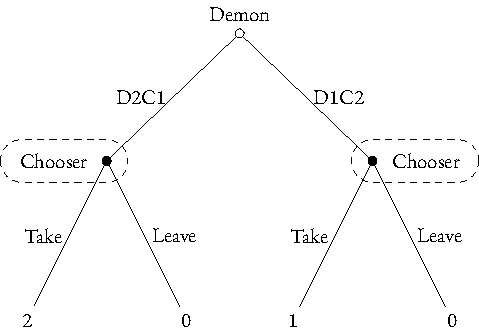
\includegraphics{fourprob-late-2024_files/figure-pdf/fig-ultimatum-1.pdf}

}

\caption{\label{fig-ultimatum}Simplified Ultimatum.}

\end{figure}%

In this game, Respondant has four possible strategies. I'll write XY for
responding to P1 with X and P2 with Y. So the strategy RA is the (odd)
strategy of rejecting the offer of \$2 and accepting the offer of \$1.
Using this terminology, this version of Ultimatum is given by
Table~\ref{tbl-ultimatum}. (As usual, I'll write the payouts for row
first, even though in this case they move second.)

\begin{longtable}[]{@{}rcc@{}}
\caption{Ultimatum game}\label{tbl-ultimatum}\tabularnewline
\toprule\noalign{}
& \textbf{P1} & \textbf{P2} \\
\midrule\noalign{}
\endfirsthead
\toprule\noalign{}
& \textbf{P1} & \textbf{P2} \\
\midrule\noalign{}
\endhead
\bottomrule\noalign{}
\endlastfoot
\textbf{AA} & \$1, \$2 & \$2, \$1 \\
\textbf{AR} & \$2, \$1 & \$0, \$0 \\
\textbf{RA} & \$0, \$0 & \$1, \$2 \\
\textbf{RR} & \$0, \$0 & \$0, \$0 \\
\end{longtable}

Assuming both players prefer more money to less, there are three Nash
equilibria of this game: (P2, AA), (P2, RA), and (P1, AR). But there is
only one dynamic equilibrium of the game: (P2, AA). In a one-shot
version of the dynamic game, there is no payoff to ever playing R; it's
always a choice between more money and less. So Respondent must play AA,
and so Proposer is best off playing P2.

Let's bring this back to decision theory. Assume that Respondent is
Chooser, our main subject. Assume also that Proposer is Demon, the
familiar character from Newcomb's Problem. Demon, as I'll understand
him, is arbitrarily good at predicting Chooser's \emph{strategy}, and
Chooser knows this.\footnote{If we wanted realistic cases, we would make
  Demon only somewhat good at predicting strategies. It would still be
  possible to get versions of most of the examples here working, but
  they would be more complicated and harder to follow. Making Demon
  arbitrarily good loses some realism, but gains some simplicity.}

Some decisions theories say that this version of Ultimatum violates
Dynamic-Strategic Equivalence (hereafter, just Equivalence). Causal
decision theorists that say Chooser should pick the optimal equilibrium,
e.g., Harper (\citeproc{ref-Harper1984}{1985}) say that Chooser should
play AR in the strategic game, but AA in the dynamic game. Evidential
decision theorists, e.g., Ahmed (\citeproc{ref-Ahmed2014}{2014}), say
the same thing.

I'm going to ultimately reject these theories, but not because of what
they say about this case. It is not obvious whether Dynamic-Strategic
Equivalence should hold here. As I just noted, some approaches to game
theory say that it should not.\footnote{I think Equivalence does hold
  here because in the strategic game AA is the only option that is not
  weakly dominated. But I'm not going to argue for weak dominance in
  this paper, or work out just how it relates to Equivalence in the
  general case. Here, as often in this paper, I'm indebted to Stalnaker
  (\citeproc{ref-Stalnaker1999}{1999}).}

There is a narrower class of decision problems where Equivalence does
seem intuitively compelling. A strategy in Table~\ref{tbl-ultimatum} is
a pair of conditionals. The strategy says what to do if Demon plays P1,
and what to do if Demon plays P2. Consider the class of decision
problems where a strategy is a single conditional. A strategy in such a
problem says \emph{If we get to this point, do X}. I call these Single
Choice problems. Here's the first statement of the core premise of this
paper.

\begin{description}
\tightlist
\item[Single Choice Principle (SCP)]
In all Single Choice problems, Dynamic-Strategic Equivalence holds.
\end{description}

The intuition behind SCP is simple. In a dynamic Single Choice game, the
only option is what to do at the point choice is called for. Assume X is
a rational move to make at that point. Now think about whether the
strategy \emph{If I reach that point, do X} is rational. Following
Ramsey (\citeproc{ref-RamseyGeneralProp}{{[}1929{]} 1990}), the way to
answer that question is to imagine reaching the point, then asking
whether it is rational to do X. And we just said that it is. So the
strategy is rational. Conversely, if doing X at that point is not
rational in the dynamic game, the same argument will show that the
strategy \emph{If I reach that point, do X} is not rational.

\section{Clarifying the Single Choice Principle}\label{sec-scp-clarify}

Think back to games involving cards. Imagine our hero, Chooser, is
playing a game in which someone else has just drawn a card. In some
sense, the game state is different if the card is an Ace than if it is a
King. But Chooser's strategy cannot depend on that. Chooser can only
react to what they know. So Chooser's strategy cannot be a list of
things about what to do at every game state, in this sense of game
state, where they have to choose.

The standard way game theorists handle this involves the notion of
\emph{information sets}. Say that the different \emph{nodes} of the game
are individuated finely enough that they encode everything that has
happened to that point which could make a difference to the outcome. So
if the other person drew an Ace, that will move the game to a different
node than if they drew a King. Say that some nodes are in the same
information set if (a) the same person must choose at every node in the
set, and (b) at any node in the set, every other node in the set is
compatible with that chooser's information at the time of
choice.\footnote{There is an implicit assumption here that epistemic
  possibility is an equivalence relation. That's too strong and for some
  purposes should be relaxed. It is, however, a harmless enough
  idealisation for the purposes of this paper.} To continue our card
game, if the other player draws a King rather than an Ace, then Chooser
has to move, those moves will take place at different nodes in the same
information set.

This terminology allows for a more perspicuous formulation of SCP.

\begin{description}
\tightlist
\item[Single Choice Principle]
Any decision problem where all the nodes where Chooser must choose are
in a single information set, Dynamic-Strategic Equivalence holds.
\end{description}

I'll work through some examples where SCP applies, and then note an
example where it does not.

Here is a rather boring game. A card will be drawn, and not shown to
Chooser. If it is neither and Ace nor a King, the game ends, as a draw.
(When a game ends, I always assume this is announced to all players.)
Otherwise, Chooser is asked to guess whether it is an Ace or a King. If
they guess correctly, they win, otherwise, they lose. The game tree for
this game is Figure~\ref{fig-ace-king}.

\begin{figure}

\centering{

\includegraphics{fourprob-late-2024_files/figure-pdf/fig-ace-king-1.png}

}

\caption{\label{fig-ace-king}The Ace-King game.}

\end{figure}%

The dashed lines around the two nodes on the right indicates that they
are in the same information set. There are two nodes where Chooser must
choose, but they are in the same information set, so SCP applies. In
this case, SCP is hardly controversial. Either guess is equally rational
in the tree in Figure~\ref{fig-ace-king}, and either guess is equally
rational in the strategic form of the game shown in
Table~\ref{tbl-ace-king}.

\begin{longtable}[]{@{}rccc@{}}
\caption{Strategic form of Ace-King
game}\label{tbl-ace-king}\tabularnewline
\toprule\noalign{}
& \textbf{Other} & \textbf{Ace} & \textbf{King} \\
\midrule\noalign{}
\endfirsthead
\toprule\noalign{}
& \textbf{Other} & \textbf{Ace} & \textbf{King} \\
\midrule\noalign{}
\endhead
\bottomrule\noalign{}
\endlastfoot
\textbf{Guess Ace} & 0 & 1 & -1 \\
\textbf{Guess King} & 0 & -1 & 1 \\
\end{longtable}

Another kind of game where SCP applies is exemplified by Newcomb's
Problem. The standard vignette that goes with Newcomb's Problem suggests
it is a dynamic choice problem. Demon \emph{predicts} what Chooser will
do, and Chooser \emph{then} selects one box or two. The fact that
Demon's predictions changes the content of an \emph{opaque} box means
that the different moves Demon could make lead to different nodes in the
same information set. All this is shown in Figure~\ref{fig-newcomb}.

\begin{figure}

\centering{

\includegraphics{fourprob-late-2024_files/figure-pdf/fig-newcomb-1.png}

}

\caption{\label{fig-newcomb}Newcomb's Problem.}

\end{figure}%

But while this is the standard vignette, it is not the way Newcomb's
Problem is usually represented. Rather, Newcomb's Problem is usually
represented in a table like Table~\ref{tbl-newcomb}, which is a correct
representation of the strategic form of Figure~\ref{fig-newcomb}.

\begin{longtable}[]{@{}rcc@{}}
\caption{Strategic form of Newcomb's
Problem}\label{tbl-newcomb}\tabularnewline
\toprule\noalign{}
& \textbf{P1} & \textbf{P2} \\
\midrule\noalign{}
\endfirsthead
\toprule\noalign{}
& \textbf{P1} & \textbf{P2} \\
\midrule\noalign{}
\endhead
\bottomrule\noalign{}
\endlastfoot
\textbf{Choose 1} & 1000 & 0 \\
\textbf{Choose 2} & 1001 & 1 \\
\end{longtable}

In tables like Table~\ref{tbl-newcomb}, I'll typically have Demon select
the column, and I'll write PX to mean that the Demon predicted X. So
here, `P1' means Demon predicted Chooser would take 1 box.

There is rather a lot of dispute about Newcomb's Problem. To the best of
my knowledge, no party to that dispute says that the difference between
Figure~\ref{fig-newcomb} and Table~\ref{tbl-newcomb} makes a difference
to that dispute. Everyone moves freely between them. This is evidence
that everyone accepts SCP restricted to Newcomb's Problem. If such a
restricted form of SCP holds, then it probably holds somewhat more
broadly. (At the very least, it should still hold if we change the
payoffs.)

So far I've shown how SCP can apply to cases involving gambles, and to
cases involving Demons. The most important applications will involve
mixing those things. In particular, we'll be interested in cases like
Figure~\ref{fig-main-example}.

Figure~\ref{fig-main-example} is a three stage decision problem. At
stage 3, if we get that far, Chooser will select Up or Down. At stage 1,
Demon will predict what Chooser will do at stage 3, again if we get that
far. At stage 2, if Demon predicts Down, nothing happens and we move to
stage 3. But if Demon predicts Up, a fair coin will be flipped. If it
lands Heads, the game ends, and Chooser gets 0. If it lands Tails, we
move to stage 3. Then after Chooser makes their choice, the payouts are
delivered. Chooser gets nothing if Demon predicted incorrectly; gets 6
if Demon correctly predicted Up, and 4 if Demon correctly predicted
Down.

\begin{figure}

\centering{

\includegraphics{fourprob-late-2024_files/figure-pdf/fig-main-example-1.png}

}

\caption{\label{fig-main-example}The main example of this paper.}

\end{figure}%

There is only 1 chice point for Chooser, so the strategy table for
Figure~\ref{fig-main-example} is very simple. It is shown in
Table~\ref{tbl-main-example}.

\begin{longtable}[]{@{}
  >{\raggedleft\arraybackslash}p{(\columnwidth - 8\tabcolsep) * \real{0.2115}}
  >{\centering\arraybackslash}p{(\columnwidth - 8\tabcolsep) * \real{0.1923}}
  >{\centering\arraybackslash}p{(\columnwidth - 8\tabcolsep) * \real{0.2115}}
  >{\centering\arraybackslash}p{(\columnwidth - 8\tabcolsep) * \real{0.1923}}
  >{\centering\arraybackslash}p{(\columnwidth - 8\tabcolsep) * \real{0.1923}}@{}}
\caption{Strategy table for
Figure~\ref{fig-main-example}}\label{tbl-main-example}\tabularnewline
\toprule\noalign{}
\begin{minipage}[b]{\linewidth}\raggedleft
\end{minipage} & \begin{minipage}[b]{\linewidth}\centering
\textbf{H} ∧ \textbf{PU}
\end{minipage} & \begin{minipage}[b]{\linewidth}\centering
\textbf{H} ∧ \textbf{PD}
\end{minipage} & \begin{minipage}[b]{\linewidth}\centering
\textbf{T} ∧ \textbf{PU}
\end{minipage} & \begin{minipage}[b]{\linewidth}\centering
\textbf{T} ∧ \textbf{PD}
\end{minipage} \\
\midrule\noalign{}
\endfirsthead
\toprule\noalign{}
\begin{minipage}[b]{\linewidth}\raggedleft
\end{minipage} & \begin{minipage}[b]{\linewidth}\centering
\textbf{H} ∧ \textbf{PU}
\end{minipage} & \begin{minipage}[b]{\linewidth}\centering
\textbf{H} ∧ \textbf{PD}
\end{minipage} & \begin{minipage}[b]{\linewidth}\centering
\textbf{T} ∧ \textbf{PU}
\end{minipage} & \begin{minipage}[b]{\linewidth}\centering
\textbf{T} ∧ \textbf{PD}
\end{minipage} \\
\midrule\noalign{}
\endhead
\bottomrule\noalign{}
\endlastfoot
\textbf{Up} & 0 & 0 & 6 & 0 \\
\textbf{Down} & 0 & 4 & 0 & 4 \\
\end{longtable}

The SCP says that the rationally acceptable moves in
Figure~\ref{fig-main-example} and Table~\ref{tbl-main-example} are the
same. If this wasn't true, we'd get a very weird result. If some
strategy is rational in Table~\ref{tbl-main-example} but not
Figure~\ref{fig-main-example}, then it would be rational for Chooser to
think \emph{If I have to choose, I'm doing X}, and then, after learning
that they have to choose and nothing else, it would be irrational to do
X. Alternatively, if some move X is rational in
Figure~\ref{fig-main-example} but not in Table~\ref{tbl-main-example},
it would be irrational to think \emph{If I have to choose, I'll do X},
even though, after learning that they had to choose and nothing else, it
would be rational to do X. Either way, this seems to violate some
fundamental rules about how conditionals work.

So, I conclude, SCP is correct. It follows from simple principles about
conditionals, and it explains why, although everything else about
Newcomb's Problem has been contested, no one has argued that the
difference in representation between Figure~\ref{fig-newcomb} and
Table~\ref{tbl-newcomb} matters.

Further, SCP is consistent with every decision rule in standard game
theory. Introductory game theory textbooks describe many `solution
concepts' for games, from avoiding dominated strategies to refinements
of Bayesian Perfect Equilibrium. All of them are consistent with SCP.

If we try strengthening SCP in natural ways, we get something
inconsistent with standard approaches to game theory. Consider, for
instance, the Single Turn Principle (hereafter, STP).

\begin{description}
\tightlist
\item[Single Turn Principle]
In any decision problem where Chooser is guaranteed to have at most one
turn, i.e., to make at most one choice between the start and the end of
the problem, Dynamic-Strategic Equivalence holds.
\end{description}

STP is strictly stronger than SCP. STP clearly entails SCP, but it rules
out choosing strategy AR in Table~\ref{tbl-ultimatum}. In the dynamic
version of that problem, Figure~\ref{fig-ultimatum}, strategy AA is
best. So even though in this game Chooser only has one turn, theories
which say AR is acceptable violate the STP. This includes the rule that
says any strategy which is part of a Nash equilibrium is choice-worthy.
So STP is inconsistent with some familiar game theoretic
approaches.\footnote{As noted earlier, it's also inconsistent with
  several decision theories, but that's a feature it shares with SCP.}

I'm making an assumption here that I will make throughout, namely that
moves in a dynamic game must be justifiable looking forward. A move at a
node in a problem must make sense given Chooser's decision theory, and
given just the facts about Chooser's beliefs about the state of the
game, and the likely outcomes given each move. This isn't a trivial
assumption, it rules out views like Functional Decision Theory
(\citeproc{ref-LevinsteinSoares2020}{Levinstein and Soares 2020}), but I
have two reasons for making the assumption.

One is simply space concerns; arguing against views like Functional
Decision Theory would take some time, and brings in wholly different
considerations.\footnote{In a longer version of this paper, I argue that
  Functional Decision Theory has very unintuitive results in cases where
  Demon is a bit less than 100\% reliable.} The other is that it is very
intuitive that in a one-shot version of Figure~\ref{fig-ultimatum},
where Chooser/Respondant has to choose between getting more money or
less money, they should choose getting more money.

This is not to assume that decision making in dynamic settings should be
entirely forward looking. Indeed, in Section~\ref{sec-dynamic} I'll
argue against that assumption. It is to assume that if forward looking
considerations imply that only one choice is rational, e.g., that
Chooser knows they'll get \$1 with one choice and \$0 with the other and
they prefer more money to less, that choice must be made.

So I'm not assuming STP; it would rule out too much in game theory. I
am, however, going to take SCP as given in what follows. It turns out to
rule out quite a bit in decision theory.

\section{Problem 1: Risk-Sensitivity}\label{sec-buchak}

Think about what value of \emph{x} would make Chooser indifferent
between these two options, and why that would be the right value:

\begin{enumerate}
\def\labelenumi{\arabic{enumi}.}
\tightlist
\item
  \$1,000,000
\item
  A gamble that returns \$2,000,000 with probability \emph{x}, and \$0
  with probability 1-\emph{x}.
\end{enumerate}

What factors are relevant to solving for \emph{x}? One factor is the
declining marginal utility of money. Money primarily has exchange value,
and if Chooser won \$2,000,000, Chooser would exchange the second
million for things they chose not to exchange the first million for, so
the second million has less value. That's one reason that \emph{x} is
well above ½.

But is it the only reason? The orthodox answer is that it is. Lara
Buchak (\citeproc{ref-BuchakRisk}{2013}) has argued that it is not. We
also need to know how much Chooser values, or more likely disvalues,
risk. That is, we need to know how risk-seeking, or risk-averse, Chooser
is.

The orthodox view is that all we need to know are three numbers. In what
follows, let \emph{b} be Chooser's current wealth in millions, and V the
function from wealth (in millions), to utility. Since V is only
determined up to positive affine transformations, we can stipulate two
of these values for V.

\begin{itemize}
\tightlist
\item
  V(\emph{b}), stipulated to be 0.
\item
  V(\emph{b} + 1), stipulated to be 1.
\item
  V(\emph{b} + 2), which we'll label \emph{c}.
\end{itemize}

On the standard view, the gamble's value is \emph{cx}, so Chooser is
indifferent between it and the money iff \emph{x}~=~1/\emph{c}. On
Buchak's view, rational Chooser has a risk function \emph{f}, that
measures their sensitivity to risk. The function must be monotonic
increasing, with \emph{f}(0)~=~0, and \emph{f}(1)~=~1. If Chooser is
risk-averse, then typically \emph{f}(\emph{x})~\textless~\emph{x}.
Buchak's view reduces to the orthodox view if
\emph{f}(\emph{x})~=~\emph{x}. I'm going to argue that given SCP,
\emph{f}(\emph{x}) does equal \emph{x}. I'm far from the first to argue
for \emph{f}(\emph{x})~=~\emph{x}.\footnote{See Briggs
  (\citeproc{ref-Briggs2015}{2015}) and Thoma
  (\citeproc{ref-Thoma2019}{2019}) for different arguments to the same
  conclusion.} What's novel here is drawing this conclusion from just
SCP.

The core of Buchak's theory is a non-standard way of valuing a gamble.
For simplicity, we'll focus on gambles with finitely many outcomes.
Associate a gamble with a random variable \emph{O}, which takes values
\emph{o}\textsubscript{1}, \ldots, \emph{o\textsubscript{n}}, where
\emph{o\textsubscript{j}}~\textgreater~\emph{o\textsubscript{i}} iff
\emph{j}~\textgreater~\emph{i}. Buchak says that the risk-weighted
expected utility of \emph{O} is given by this formula, where \emph{f} is
the agent's risk-weighting function.

\begin{quote}
REU(\emph{O}) = \emph{o}\textsubscript{1} + \(\sum_{i = 2}^n\)
\emph{f}(Pr(\emph{O} ⩾
\emph{o\textsubscript{i}}))(\emph{o\textsubscript{i}} -
\emph{o}\textsubscript{\emph{i}-1})
\end{quote}

The decision rule then is simple: choose the gamble with the highest
REU. The key notion here is the risk function \emph{f}, which we
introduced earlier. I'm going to show that if
\emph{f}(\emph{x})~=~\emph{x}\textsuperscript{2}, then we get a
violation of SCP. I won't go through the details of how this generalises
to all other values of \emph{f} other than identity\footnote{If \emph{f}
  is the identity function, Buchak's way of valuing gambles just becomes
  orthodox expected utility theory.}, but it should be easy enough to
see how to use the recipe here to find a problem for any other value of
\emph{f}.

As is standard, I'll assume that random moves in a game are made by a
player called Nature. Chooser is always assumed to know the moves
available to Nature at a node, and the probability that it will make any
given move having arrived at that node.

In Figure~\ref{fig-buchak} at stage 1 a fair die will be rolled. If it
lands 1 or 2, Nature moves Left; if it lands 3 or 4, Nature moves
Middle; otherwise, Nature moves Right. If Nature moves Left, the game
ends, and Chooser gets 1. Otherwise Chooser is told that Nature did not
move Left, but not whether they moved Middle or Right. If Chooser
selects Down, they get 1. If Chooser selects Up, they get 5 if Nature
moved Middle, and 0 otherwise.

\begin{figure}

\centering{

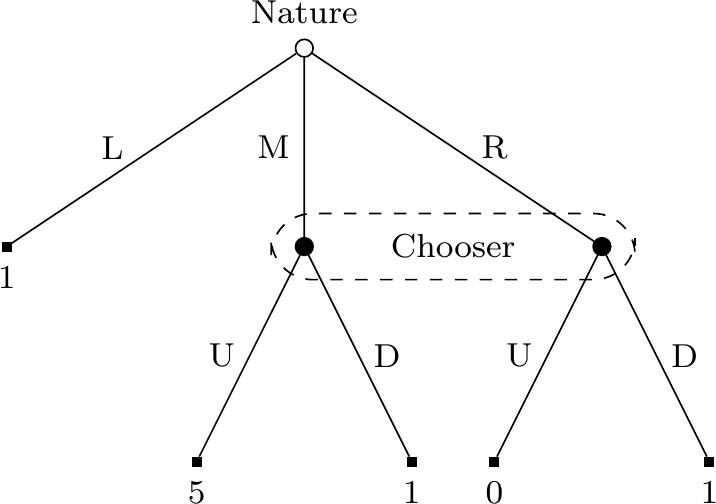
\includegraphics{fourprob-late-2024_files/figure-pdf/fig-buchak-1.png}

}

\caption{\label{fig-buchak}Tree Diagram of the counterexample to REU.}

\end{figure}%

Table~\ref{tbl-buchak-early} shows the strategic table of
Figure~\ref{fig-buchak}, and Table~\ref{tbl-buchak-late} shows the
decision table Chooser faces at the time they have to choose.

\begin{table}

\caption{\label{tbl-panel}Two strategy tables for
Figure~\ref{fig-buchak}.}

\begin{minipage}{0.50\linewidth}

\subcaption{\label{tbl-buchak-early}The strategy table at game start.}

\centering{

\begin{tabular}{cccc}
\toprule
 & \textbf{Left} & \textbf{Middle} & \textbf{Right}\\
\midrule
\textbf{Up} & 1 & 5 & 0\\
\textbf{Down} & 1 & 1 & 1\\
\bottomrule
\end{tabular}

}

\end{minipage}%
%
\begin{minipage}{0.50\linewidth}

\subcaption{\label{tbl-buchak-late}The strategy table at choice time.}

\centering{

\begin{tabular}{ccc}
\toprule
 & \textbf{Middle} & \textbf{Right}\\
\midrule
\textbf{Up} & 5 & 0\\
\textbf{Down} & 1 & 1\\
\bottomrule
\end{tabular}

}

\end{minipage}%

\end{table}%

In Table~\ref{tbl-buchak-early}, the REU of Down is 1 (since that's the
only possible outcome), and the REU of Up is 8/9. There is a 2/3 chance
of getting at least 1, so that's worth 4/9, and there's a 1/3 chance of
getting another 4, so that's also worth 4/9, and adding those gives 8/9.
So the optimal strategy, according to REU theory, is Down. That is, REU
says to prefer the strategy \emph{Choose Down if you have to choose} to
the strategy \emph{Choose Up if you have to choose}. But if we get to
the choice point, we're at Table~\ref{tbl-buchak-late}. And in that
table the REU of Up is 5 times 1/4, i.e., 5/4. So at that point, REU
says to choose Up. What REU says to do if you have to choose is
different to which strategy it chooses for the one and only point you
have to choose at. That is, Buchak's theory violates the SCP, and so
should be rejected.

\section{Problem 2: Demons and Multiple Equilibria}\label{sec-multiple}

This section is about problems like Newcomb's Problem
(\citeproc{ref-Nozick1969}{Nozick 1969}). I'm not going to start with
Newcomb's Problem itself; I would end up replaying familiar lines if I
started there. Instead I'll start with a very generic form of similar
problems.

Table~\ref{tbl-generic-demon} is (the strategic form of) a completely
generic form of a 2-by-2 decision problem involving demons. At stage 2,
Chooser will pick Up or Down. At stage 1, Demon will predict what
Chooser will do. I'll only discuss cases where Demon is (believed to be)
arbitrarily close to perfect in their predictions.

\begin{longtable}[]{@{}ccc@{}}
\caption{A generic demon
problem.}\label{tbl-generic-demon}\tabularnewline
\toprule\noalign{}
& \textbf{PU} & \textbf{PD} \\
\midrule\noalign{}
\endfirsthead
\toprule\noalign{}
& \textbf{PU} & \textbf{PD} \\
\midrule\noalign{}
\endhead
\bottomrule\noalign{}
\endlastfoot
\textbf{Up} & \emph{a} & \emph{b} \\
\textbf{Down} & \emph{c} & \emph{d} \\
\end{longtable}

Say that an option is a strict equilibrium if, assuming Demon predicts
correctly, Chooser's payout for choosing it is (strictly) greater than
their payout for choosing any other option. So Up is a strict
equilibrium if \emph{a}~\textgreater~\emph{c}. The focus in this section
is going to be on problems where both Ip and Down are strict equilibria,
so \emph{a}~\textgreater~\emph{c}, and \emph{d}~\textgreater~\emph{b}.
While Newcomb's Problem itself is not such a case, most of the views
that have been proposed to deal with Newcomb's Problem have consequences
for the case where both Up and Down are strict equilibria, and they
typically say things that violate SCP.

To simplify matters, I'm going to make two further assumptions which are
widely, but not universally, shared. First, I'll assume that the names
of the options are irrelevant. In particular, I'll assume that if Up is
rationally permissible in Table~\ref{tbl-generic-demon}, then Down is
permissible in Table~\ref{tbl-inverted-generic}. Call this assumption
\textbf{Label Neutrality}.

\begin{longtable}[]{@{}ccc@{}}
\caption{Table~\ref{tbl-generic-demon} with labels
inverted.}\label{tbl-inverted-generic}\tabularnewline
\toprule\noalign{}
& \textbf{PU} & \textbf{PD} \\
\midrule\noalign{}
\endfirsthead
\toprule\noalign{}
& \textbf{PU} & \textbf{PD} \\
\midrule\noalign{}
\endhead
\bottomrule\noalign{}
\endlastfoot
\textbf{Up} & \emph{d} & \emph{c} \\
\textbf{Down} & \emph{b} & \emph{a} \\
\end{longtable}

The second assumption is that in any instance of
Table~\ref{tbl-generic-demon}, the four payouts, plus the conditional
probabilities of a correct prediction given each choice by Chooser,
settle which options are choice-worthy. This isn't universally shared,
but it is very widely shared. Indeed, it is common in philosophy papers
to specify nothing but these values and then ask for intuitions about
the case, which suggests many people do presuppose that only these
values are necessary. Call this assumption \textbf{Settling}, because
the values (plus the probabilities of correct prediction given each
choice) settle what is choice-worthy.

\textbf{Settling} is rejected by theorists such as Skyrms
(\citeproc{ref-Skyrms1982}{1982}) and Joyce
(\citeproc{ref-Joyce2012}{2012}), who say that in problems like these,
Chooser's starting view about what option they will eventually select
also makes a difference to what they should do. Those views are not
subject to the objections I'm about to make----provided Chooser's
credences satisfy some rather tight constraints.

I'm going to largely focus on versions of Table~\ref{tbl-generic-demon}
where \emph{a} and \emph{d} are positive, and \emph{b}~=~\emph{c}~=~0.
This kind of problem is called Nice Demon by Skyrms
(\citeproc{ref-Skyrms1982}{1982}) and Weirich
(\citeproc{ref-Weirich1988}{1988}), and is shown in
Table~\ref{tbl-nice-demon}. I'm going to mostly discuss the case,
discussed by Weirich but not Skyrms, where \emph{a}~≠~\emph{d}. The main
conclusion is that given these three assumptions (SCP, \textbf{Label
Neutrality} and \textbf{Settling}), both Up and Down are permissible in
these cases.

\begin{longtable}[]{@{}ccc@{}}
\caption{Nice demon.}\label{tbl-nice-demon}\tabularnewline
\toprule\noalign{}
& \textbf{PU} & \textbf{PD} \\
\midrule\noalign{}
\endfirsthead
\toprule\noalign{}
& \textbf{PU} & \textbf{PD} \\
\midrule\noalign{}
\endhead
\bottomrule\noalign{}
\endlastfoot
\textbf{Up} & \emph{a} & 0 \\
\textbf{Down} & 0 & \emph{d} \\
\end{longtable}

There is a quick argument, independent of SCP, for the same conclusion.
Whatever values \emph{a} and \emph{d} are, it's permissible for Chooser
to be arbitrarily confident that they will play Up. Given that
confidence, Chooser should think that Up maximises expected utility.
It's permissible to choose an option that maximises expected utility
given permissible credences. Therefore Up is rationally permissible.
Since Up was arbitrary in this argument, it is also permissible to
choose Down, so both are permissible.

Weirich (\citeproc{ref-Weirich1988}{1988, 563}) makes a version of this
argument, and then says that since the conclusion is obviously false,
something must be wrong with it. He thinks that Chooser should not be
allowed to use credences about their own future actions in the way the
argument presupposes. This allows him to say, along with many others,
that if \emph{d}~\textgreater~\emph{a}, then only Down is rationally
permissible. I'm not going to rely on this argument, but simply note
that it doesn't seem like a bad argument to me, and in any case I will
be endorsing its conclusion.\footnote{Spencer
  (\citeproc{ref-Spencer2023}{2023}) makes a related argument in the
  course of defending the permissibility of both options.}

There are three interesting families of views which differ markedly with
each other in general, but which agree that in
Table~\ref{tbl-nice-demon}, whichever of \emph{a} and \emph{d} is larger
determines which option is uniquely choiceworthy.

The first family of views is just a single, famous, view: Evidential
Decision Theory. It says that in any version of
Table~\ref{tbl-generic-demon}, if \emph{a}~≠~\emph{d}, then whichever is
larger should be chosen. Hence it says that in
Table~\ref{tbl-nice-demon}, the larger value should be chosen.

The second family of views are what Eells and Harper
(\citeproc{ref-EellsHarper1991}{1991}) call Maximum Ratifiability views.
They say that when there are multiple ratifiable options, the value with
the highest expected utility should be chosen. Such views differ on what
to do when there are no ratifiable options, which is why I'm calling
this a family of views. But they all agree on
Table~\ref{tbl-nice-demon}. Maximum Ratifiability is defended by Jeffrey
(\citeproc{ref-Jeffrey1983}{1983}), Sobel
(\citeproc{ref-Sobel1983}{1983}), Harper
(\citeproc{ref-Harper1984}{1985}), Weirich
(\citeproc{ref-Weirich1988}{1988}), Arntzenius
(\citeproc{ref-Arntzenius2008}{2008}), and Gustafsson
(\citeproc{ref-Gustafsson2011}{2011}).

The third family of views say that in any version of
Table~\ref{tbl-generic-demon}, one should minimise possible regret. That
is, one should choose Up if the possible Regret from choosing Up,
\emph{d}~-~\emph{b}, is less than the possible regret from choosing
Down, \emph{a}~-~\emph{c}. Wedgwood
(\citeproc{ref-Wedgwood2013a}{2013}), Gallow
(\citeproc{ref-Gallow2020}{2020}), Podgorski
(\citeproc{ref-Podgorski2022}{2022}), and Barnett
(\citeproc{ref-Barnett2022}{2022}) endorse such a view, though they go
on to say very different things about cases with three or more options.
These views also say that in Table~\ref{tbl-nice-demon}, whichever of
\emph{a} and \emph{d} is larger determines the uniquely choiceworthy
option.

All of these views violate SCP. The argument turns on the problem
depicted in Figure~\ref{fig-main-example}, back in
Section~\ref{sec-scp-clarify}. Recall that it's a three stage decision
problem.

\begin{itemize}
\tightlist
\item
  First, Demon predicts what Chooser will do at stage three (if it gets
  that far).
\item
  Second, if Demon predicts Up, a coin will be flipped. If it lands
  Heads, the problem ends, and Chooser gets 0. Otherwise we continue to
  stage three.
\item
  Third, Chooser chooses Up or Down. If Demon's prediction is incorrect,
  Chooser gets 0. But that's unlikely; Demon is arbitrarily good at
  predictions. If Demon correctly predicted Up, Chooser gets 6; if Demon
  correctly predicted Down, Chooser gets 4.
\end{itemize}

All of the views just described say that, if it reaches stage three,
Chooser should take Up. At that time, Up maximises conditional expected
utility, it has the highest return of any ratifiable option, and it
minimises possible regret.

The strategic form of the problem is given in
Table~\ref{tbl-main-example-simple}. I'd previously given the strategic
form of the problem as \#tbl-main-example, but now it can be simplified.
That's because we've shown (in Section~\ref{sec-buchak}) that Chooser
should maximise expected utility, not risk-adjusted expected utility.

\begin{longtable}[]{@{}rcc@{}}
\caption{Simplified strategic form of
Figure~\ref{fig-main-example}.}\label{tbl-main-example-simple}\tabularnewline
\toprule\noalign{}
& \textbf{PU} & \textbf{PD} \\
\midrule\noalign{}
\endfirsthead
\toprule\noalign{}
& \textbf{PU} & \textbf{PD} \\
\midrule\noalign{}
\endhead
\bottomrule\noalign{}
\endlastfoot
\textbf{Up} & 3 & 0 \\
\textbf{Down} & 0 & 4 \\
\end{longtable}

In this example, Down is uniquely choice-worthy on all three of these
theories. It maximises conditional expected utility, it is the
ratifiable choice with maximum return, and it minimises possible regret.

So all of these views violate the SCP. In the strategic form of
Figure~\ref{fig-main-example}, they prefer Down to Up, but at the only
point Chooser can possibly move in Figure~\ref{fig-main-example}, they
prefer Up to Down.

The point is not that this leads to any kind of Dutch Book, or money
pump, or sure loss. Any attempt to turn the SCP into a pragmatic
argument like this would fail. Rather, it is that these views answer the
same question two different ways, depending on how it is asked. As David
Christensen (\citeproc{ref-Christensen1996}{1996}) argued, this is
really what's significant in Dutch Book arguments.

The two questions that they are answering differently are:

\begin{enumerate}
\def\labelenumi{\arabic{enumi}.}
\tightlist
\item
  Do you prefer that, if Chooser reaches stage 3, they play Up or Down?
\item
  On the assumption that Chooser reaches stage 3, do you prefer they
  play Up or Down?
\end{enumerate}

The answer they give to Q1 is \emph{Down}.that follows from the fact
that they prefer Down to Up in Table~\ref{tbl-main-example-simple}. The
answer they give to Q2 is \emph{Up}. that follows from the fact that
they prefer Up to Down if we replace the 3 in
Table~\ref{tbl-main-example-simple} with the actual payout for a correct
prediction of Up, namely 6.

Now one could try to develop a theory of conditionals on which it makes
sense to answer these questions differently. Or one could try to develop
a metaphysics of strategies that undermined a background assumption of
this paper, namely that we should express strategies as conditionals. I
suspect the prospects for either approach are dim, and so I think this
is an argument that all of these views are incoherent; they give
inconsistent answers to two formulations of the very same question.

\section{General Ratifiability}\label{sec-general-ratify}

In the previous section I argued that in any instance of Nice Demon,
where Chooser gets a reward iff Demon's prediction is correct, both
options are choice-worthy. In this section I generalise that result. In
any instance of \#tbl-generic-demon where both choices are strict
equilibria, both options are choiceworthy.\footnote{I'm grateful to
  Dmitri Gallow for suggestions which greatly strengthened and
  simplified the proof that follows.}

The proof relies on five assumptions, three of which were used in the
last section: SCP, \textbf{Label Neutrality} and \textbf{Settling}.

The fourth assumption is that the values in the table are utilities, and
hence are only unique up to positive affine transformation. So whatever
choices are rational in a table, the same choices are rational if each
payout is multiplied by a positive constant, and/or some (other
constant) is added. Call this assumption \textbf{Affine
Transformtation}.

The fifth and final assumption is that in two option decision problems
with two strict equilibria, at least one (pure) option is choice-worthy.
That is, these problems are not dilemmas (even if Chooser only plays
pure strategies).

Given those assumptions, we'll show that both options are choice-worthy
in two option problems where both options are strict equilibria. It
simplifies the proof a little to work not with
Table~\ref{tbl-generic-demon}, but with a slightly relabeled version, as
shown in Table~\ref{tbl-two-good}.

\begin{longtable}[]{@{}ccc@{}}
\caption{A problem with two strict
equilibria.}\label{tbl-two-good}\tabularnewline
\toprule\noalign{}
& \textbf{PU} & \textbf{PD} \\
\midrule\noalign{}
\endfirsthead
\toprule\noalign{}
& \textbf{PU} & \textbf{PD} \\
\midrule\noalign{}
\endhead
\bottomrule\noalign{}
\endlastfoot
\textbf{Up} & \emph{a} & \emph{d}-\emph{c} \\
\textbf{Down} & \emph{a}-\emph{b} & \emph{d} \\
\end{longtable}

Since the game has two strict equilibria, both \emph{b} and \emph{c} are
positive. Assume without loss of generality that \emph{a} and \emph{d}
are also positive. (If not use \textbf{Affine Transformation} to make
them both positive.) Assume, also without loss of generality, that
\emph{b}~\textgreater~\emph{c}. (If not, use \textbf{Label Neutrality}
to flip the labels.)

Consider the dynamic decision problem shown in
Figure~\ref{fig-two-good}. In this tree, we'll leave both the
probability of tails, \emph{p}, and the exit payout,
\emph{e}/(1-\emph{p}), as unknows to be solved for. (This problem
differs from Figure~\ref{fig-main-example} in that we don't assume the
coin in stage two is fair, but we do assume the probability of Heads is
known to Chooser.)

\begin{figure}

\centering{

\includegraphics{fourprob-late-2024_files/figure-pdf/fig-two-good-1.png}

}

\caption{\label{fig-two-good}A problem where if Chooser moves, they are
in Table~\ref{tbl-two-good}.}

\end{figure}%

The strategic form of Figure~\ref{fig-two-good} is given by
Table~\ref{tbl-two-good-strategic}.

\begin{longtable}[]{@{}ccc@{}}
\caption{The strategic form of
Figure~\ref{fig-two-good}.}\label{tbl-two-good-strategic}\tabularnewline
\toprule\noalign{}
& \textbf{PU} & \textbf{PD} \\
\midrule\noalign{}
\endfirsthead
\toprule\noalign{}
& \textbf{PU} & \textbf{PD} \\
\midrule\noalign{}
\endhead
\bottomrule\noalign{}
\endlastfoot
\textbf{Up} & \emph{pa} + \emph{e} & \emph{d}-\emph{c} \\
\textbf{Down} & \emph{p}(\emph{a}-\emph{b}) + \emph{e} & \emph{d} \\
\end{longtable}

By SCP, Up is choice-worthy in Table~\ref{tbl-two-good} iff Up is
choice-worthy in Table~\ref{tbl-two-good-strategic}. By \textbf{Label
Neutrality} and \textbf{Affine Transformation}, Up is choice-worthy in
Table~\ref{tbl-two-good} iff Down is choice-worthy in
Table~\ref{tbl-two-good-inverted}. (This is because we get from
Table~\ref{tbl-two-good} to Table~\ref{tbl-two-good-inverted} by first
flipping the labels, then multiplying the payouts by \emph{m} and adding
\emph{x} to every payout.)

\begin{longtable}[]{@{}ccc@{}}
\caption{Inverted and transformed version of
Table~\ref{tbl-two-good}.}\label{tbl-two-good-inverted}\tabularnewline
\toprule\noalign{}
& \textbf{PU} & \textbf{PD} \\
\midrule\noalign{}
\endfirsthead
\toprule\noalign{}
& \textbf{PU} & \textbf{PD} \\
\midrule\noalign{}
\endhead
\bottomrule\noalign{}
\endlastfoot
\textbf{Up} & \emph{md} + \emph{x} & \emph{m}(\emph{a}-\emph{b}) +
\emph{x} \\
\textbf{Down} & \emph{m}(\emph{d}-\emph{c}) + \emph{x} & \emph{ma} +
\emph{x} \\
\end{longtable}

If we can find values of \emph{p}, \emph{e}, \emph{m} and \emph{x} such
that Table~\ref{tbl-two-good-strategic} and
Table~\ref{tbl-two-good-inverted} are identical, it will follow that Up
is choice-worthy in Table~\ref{tbl-two-good} iff Down is choice-worthy.
(Note we must also check that \emph{m} is positive, and \emph{p} is a
probability, i.e., in {[}0, 1{]}.) From that plus the no dilemmas
assumption, it follows that Up and Down are both choice-worthy in
Table~\ref{tbl-two-good}, as required.

Now it's just a bit of algebra to figure out the four unknowns \emph{p},
\emph{e}, \emph{m} and \emph{x} given the four equations, i.e., the
equality of matching cells in Table~\ref{tbl-two-good-strategic} and
Table~\ref{tbl-two-good-inverted}.

\begin{align*}
(1) && pa + e &= md + x && \text{(Top left)} \\
(2) && d - c &= m(a - b) + x && \text{(Top right)} \\
(3) && p(a - b) + e &= m(d - c) + x && \text{(Bottom left)} \\
(4) && d &= ma + x && \text{(Bottom right)} \\
(5) && c &= mb && \text{(4) - (2)} \\
(6) && m &= \frac{c}{b} && \text{(5)} \\
(7) && pb &= mc && \text{(1) - (3)} \\
(8) && pb &= \frac{c^2}{b} && \text{(6), (7)} \\
(9) && p &= \frac{c^2}{b^2} && \text{(8)} \\
(10) && x &= d - c - m(a - b) && \text{(2)} \\
(11) && x &= d - c - \frac{c(a - b)}{b} && \text{(6), (10)} \\
(12) && x &= d - c - \frac{ca}{b} + c && \text{(11)} \\
(13) && x &= d - \frac{ca}{b} && \text{(12)} \\
(14) && \frac{ac^2}{b^2} + e &= \frac{dc}{b} + d - \frac{ca}{b} && \text{(1), (6), (9), (13)} \\
(15) && e &= \frac{bcd + db^2 - abc - ac^2}{b^2} && \text{(14)}
\end{align*}

Lines 6, 9, 13 and 15 give the values for the four variables. Since
\emph{b} and \emph{c} are positive, \emph{m} and \emph{p} are also
positive.\footnote{Note that all we need here is that \emph{b} and
  \emph{c} have the same sign. So this argument has consequences for the
  case where there is no pure equilibrium. But I'm setting aside those
  cases, which raise issues about mixed strategies, for this paper.}
Since \emph{b}~\textgreater~\emph{c}, \emph{p}~\textless~1, so \emph{p}
is a probability.

I won't go through all the algebra, but substituting these values for
the four variables back into either Table~\ref{tbl-two-good-strategic}
or Table~\ref{tbl-two-good-inverted} gives
Table~\ref{tbl-two-good-final}.

\begin{longtable}[]{@{}ccc@{}}
\caption{Final version of
Table~\ref{tbl-two-good}.}\label{tbl-two-good-final}\tabularnewline
\toprule\noalign{}
& \textbf{PU} & \textbf{PD} \\
\midrule\noalign{}
\endfirsthead
\toprule\noalign{}
& \textbf{PU} & \textbf{PD} \\
\midrule\noalign{}
\endhead
\bottomrule\noalign{}
\endlastfoot
\textbf{Up} & (\emph{bd} + \emph{cd} - \emph{ac})/\emph{b} & \emph{d} -
\emph{c} \\
\textbf{Down} & (\emph{bd} + \emph{cd} - \emph{ac} -
\emph{c}\textsuperscript{2})/\emph{b} & \emph{d} \\
\end{longtable}

That's enough to show, given the assumptions we started with that Up and
Down are both choice-worthy in Table~\ref{tbl-two-good}.

This doesn't yet show that any ratifiable choice is choice-worthy; it
doesn't even show anything for cases where Chooser has three options.
But it does show that SCP is inconsistent with any view that accepts the
other four assumptions, and which says that only one option is
choice-worthy in Table~\ref{tbl-two-good}. That, as I discussed in the
previous section, includes a large number of decision theories
philosophers have defended.

\section{Question 3: Incompleteness}\label{sec-incompleteness}

Standard, textbook, approaches to decision theory assume that agents
have numerical probabilities for each possible state, and numerical
values for each possible outcome. The use of numbers here is not a
trivial assumption; the real numbers have many distinct characteristics.
Among other things, they are linearly ordered. In other words, the
comparative relation between them is \emph{complete}. If \emph{x} and
\emph{y} are numbers, then either \emph{x} is larger, or \emph{y} is
larger, or they are equal. Probabilities and values are only numerically
representatable if for any two of them, either they are equal, or one is
larger.

For both probabilities and values, this completeness assumption has been
questioned. Keynes (\citeproc{ref-Keynes1921}{1921}) argued at length
against probabilities being complete. He argued probabilities must be
non-numerical because sometimes there are distinct probabilities where
neither is greater than the other. Ruth Chang
(\citeproc{ref-Chang2002}{2002}) argued that some options are `on a par'
in terms of value, and this is a state distinct from equality (or either
being better).

In this section I'll discuss a kind of non-linearity that hasn't
received as much philosophical attention. Even if probabilities and
values (of outcomes) are complete, preferences over options need not be
complete. Indeed, SCP implies that there will be some incompleteness, at
least if Demon is possible.

This is not a completely novel result. Eells and Harper
(\citeproc{ref-EellsHarper1991}{1991}) prove something similar given the
assumption that the choice-worthy options are the ratifiable ones. SCP
doesn't entail this version of ratificationism, but I think you can
probably recover the consequences of ratificationism that Eells and
Harper use as premises in their argument. I won't do that however; it's
easier to argue directly from SCP to incompleteness.

One immediate question is just how to state incompleteness. If what it
means for two options to be equally good just is that neither is
strictly preferred to the other, then completeness follows immediately
from the asymmetry of strict preference. We need some other way to
understand what it is for options to be equally preferred.

One suggestion comes from Chang. She notes that if two options are
equally good, then adding a small `sweetener' to one of them should make
the sweetened option better. If there are two options such that neither
is strictly preferred to the other, and even after sweetening one,
neither is strictly preferred to the other, then completeness fails.

Another suggestion comes from an approach to decision theory that traces
back to Samuelson (\citeproc{ref-Samuelson1938}{1938}). Some theorists
have been sceptical of the very notion of preferences over options.

Originally the motivation for this scepticism was somewhat behaviourist.
If I have fifteen options, there is no behavioural difference between
having \emph{x} as my tenth best option and \emph{y} as my eleventh, or
vice versa. I won't choose either option either way.

What makes a behavioural difference is which options I take to be
choice-worthy out of a set of options. We represent this by saying that
when X is a set of options, c(X) is the set of choice-worthy options;
they are the ones that I might (assuming I'm rational) pick.

These days behaviourist motivations are not given much weight, and
rightly so. But there are other reasons to centre decision theory around
choice functions rather than preference relations. As Sen
(\citeproc{ref-Sen1971}{1971}) shows, this formulation allows us to
easily represent various options that are a bit more awkward to
represent if we take preference as the central bit of ideology in our
theory.

Now one might think that moving from preference to choice-theory won't
help characterise incompleteness. In fact, it may make things worse.
It's natural to think that if c(\{\emph{x},~\emph{y}\})~=~\{\emph{x}\},
then \emph{x} is preferred to \emph{y}, if
c(\{\emph{x},~\emph{y}\})~=~\{\emph{y}\}, then \emph{y} is preferred to
\emph{x}, and if c(\{\emph{x},~\emph{y}\})~=~\{\emph{x}, \emph{y}\},
then each option is equally good. We'll set aside whether the first two
claims are right, and note one reason to be suspicious of the third.

If \emph{x} and \emph{y} are equally preferred, then in any larger set
of options that contains them both, either both should be choice-worthy
or neither one should be. Saying one is choice-worthy but not the other
violates the idea that they are equally good. Sen's Principle β is a
generalisation of this idea; we'll work with the simpler version.

\begin{description}
\tightlist
\item[Simplified β]
If c(\{\emph{x},~\emph{y}\})~=~\{\emph{x}, \emph{y}\}, then for any
\emph{z}: \emph{x} ∈ c(\{\emph{x},~\emph{y},~\emph{z}\}) iff \emph{y} ∈
c(\{\emph{x},~\emph{y},~\emph{z}\}).
\end{description}

Given \textbf{Simplified β}, it is plausible to equate
c(\{\emph{x},~\emph{y}\})~=~\{\emph{x}, \emph{y}\} with \emph{x} and
\emph{y} are equally good. But if \textbf{Simplified β} fails, then it
is more plausible that preferences at this point are incomplete. Indeed,
given some weak (but not quite trivial) assumptions about c, we can
prove that completeness is equivalent to \textbf{Simplified
β}.\footnote{For a careful statement of what those assumptions are, see
  Sen (\citeproc{ref-Sen1971}{1971}) or Kreps
  (\citeproc{ref-Kreps1988}{1988}).}

I just gave two ways of testing for incompleteness, but they end up
being very closely related. Assume
c(\{\emph{x},~\emph{y}\})~=~\{\emph{x}, \emph{y}\}, and let \emph{z} be
a small sweetening of \emph{x}. Perhaps it is \emph{x} plus a dollar.
Then if sweetening does not destroy the parity between \emph{x} and
\emph{y}, we'll have
c(\{\emph{x},~\emph{y},~\emph{z}\})~=~\{\emph{y},~\emph{z}\}, violating
\textbf{Simplified β}.

It's easy to show that SCP leads to cases where sweetening does not
break `ties', and where \textbf{Simplified β} fails. For both cases,
start with Table~\ref{tbl-nice-demon-linear}.

\begin{longtable}[]{@{}ccc@{}}
\caption{A version of Nice
Demon.}\label{tbl-nice-demon-linear}\tabularnewline
\toprule\noalign{}
& \textbf{PU} & \textbf{PD} \\
\midrule\noalign{}
\endfirsthead
\toprule\noalign{}
& \textbf{PU} & \textbf{PD} \\
\midrule\noalign{}
\endhead
\bottomrule\noalign{}
\endlastfoot
\textbf{Up} & 6 & 0 \\
\textbf{Down} & 0 & 4 \\
\end{longtable}

According to SCP, both Up and Down are choice-worthy in
Table~\ref{tbl-nice-demon-linear}. If we sweeten Up by adding 1 to it,
i.e., adding 1 to each payout, we get Table~\ref{tbl-nice-demon-plus}.

\begin{longtable}[]{@{}ccc@{}}
\caption{Table~\ref{tbl-nice-demon-linear} with Up
sweetened.}\label{tbl-nice-demon-plus}\tabularnewline
\toprule\noalign{}
& \textbf{PU} & \textbf{PD} \\
\midrule\noalign{}
\endfirsthead
\toprule\noalign{}
& \textbf{PU} & \textbf{PD} \\
\midrule\noalign{}
\endhead
\bottomrule\noalign{}
\endlastfoot
\textbf{Up} & 7 & 1 \\
\textbf{Down} & 0 & 4 \\
\end{longtable}

As we showed in Section~\ref{sec-general-ratify}, both Up and Down are
still choice-worthy in problems like Table~\ref{tbl-nice-demon-plus},
where both options are strict equilibria.

To get a violation of \textbf{Simplified β}, add a `safe' option to
Table~\ref{tbl-nice-demon-linear}, as in
Table~\ref{tbl-nice-demon-safe}.\footnote{For completeness, assume in
  Table~\ref{tbl-nice-demon-safe} that if Demon predicts Safe, Demon
  will flip a coin to decide whether to play PU or PD.}

\begin{longtable}[]{@{}ccc@{}}
\caption{Table~\ref{tbl-nice-demon-linear} with a safe
option.}\label{tbl-nice-demon-safe}\tabularnewline
\toprule\noalign{}
& \textbf{PU} & \textbf{PD} \\
\midrule\noalign{}
\endfirsthead
\toprule\noalign{}
& \textbf{PU} & \textbf{PD} \\
\midrule\noalign{}
\endhead
\bottomrule\noalign{}
\endlastfoot
\textbf{Up} & 6 & 0 \\
\textbf{Down} & 0 & 4 \\
\textbf{Safe} & 5 & 5 \\
\end{longtable}

In Table~\ref{tbl-nice-demon-safe}, Up is still choice-worthy, but Down
is not, since it is strictly dominated. So \textbf{Simplified β} fails.

So given SCP (and the other assumptions in
Section~\ref{sec-general-ratify}), there are cases where both options
are choice-worthy and (a) sweetening one of them still leaves both
choice-worthy, and (b) adding a third option makes one but not the other
choice-worthy. That strongly suggests this is a theory where preferences
over options are incomplete.

In Table~\ref{tbl-nice-demon-linear}, Chooser should not strictly prefer
Up to Down or vice versa, else they would not both be choice-worthy, but
nor should they think they are equally good, else we would not have
these results. So this is a case where, even though probabilities and
outcome values are complete, preferences are incomplete.

\section{Consequences of
Incompleteness}\label{consequences-of-incompleteness}

This conclusion of Section~\ref{sec-incompleteness} is relevant to the
arguments that Keynes, Chang, and others have made. Keynes, especially
in the \emph{General Theory} (\citeproc{ref-Keynes1936}{Keynes 1936}),
was interested in situations where intuitively all of the following are
true.

\begin{enumerate}
\def\labelenumi{\arabic{enumi}.}
\tightlist
\item
  The farm is not worth more than £1,000,000.
\item
  The farm is not worth less than £1,000,000.
\item
  The farm is not worth exactly £1,000,000.
\end{enumerate}

One way to argue for 3 is the small improvements argument; if the farm
is worth exactly £1,000,000, then an afternoon of slightly better than
expected weather should break the tie. But that's not how we value
farms.

One way to argue for 1 and 2 is that decisions to trade, i.e., to buy or
sell the farm for £1,000,000, seem to rely on `animal spirits'; it isn't
like anyone thinks that selling the farm for £1,000,000 is a great deal,
or that buying it for £1,000,000 is a bargain. This is a very simplified
summary of Keynes's reasoning, but let's stick with it for now.

As Dorr, Nebel, and Zuehl (\citeproc{ref-DorrEtAl2023}{2023, sec. 5})
point out, this is a pretty weak argument. At most, what this shows is
that the farm is not \emph{definitely} worth more or \emph{definitely}
worth less than £1,000,000. But it could be that the value of the farm
is vague, where this still means it is more than, less than, or equal to
£1,000,000. They suggest that all the cases where completeness
intuitively fails are like this; none of the comparative claims is
definitely true, but one is actually true.\footnote{They also have a
  direct argument for comparability turning on some intuitions about
  negated comparison claims. It would take us very far afield to go over
  that carefully, but the argument from SCP for incomparability is
  relevant here too. The cost of giving up the semantic intuitions they
  rely on seems, to me at least, much less than the cost of giving up
  the Ramsey test for conditionals. And the Ramsey test is enough to
  motivate SCP. This may be a case where the different semantic
  intuitions are inconsistent, in which case we have to see which
  intuition is least costly to abandon. Working that out in full is a
  task for another paper, but I doubt the answer is that it's best to
  abandon the Ramsey test.}

Whether that diagnosis of the intuitions that Keynes, Chang, and others
put forward is right, it won't help explain what's going on in the case
here. In Table~\ref{tbl-nice-demon-linear}, all of the following are
true.

\begin{enumerate}
\def\labelenumi{\arabic{enumi}.}
\tightlist
\item
  Up is not better (for Chooser) than Down. If it were, Down would not
  be choice-worthy.
\item
  Down is not better (for Chooser) than Up. If it were, Up would not be
  choice-worthy.
\item
  Up and Down are not equally good (for Chooser). If they were, they
  would still be equally good when a third option was added, which is
  inconsistent with the fact that Up but not Down is choice-worthy in
  Table~\ref{tbl-nice-demon-safe}.
\end{enumerate}

The arguments from SCP don't just show 1-3 are true; they show that 1-3
are definitely true. So this attempt to explain away intuitions opposing
completeness doesn't fully generalise.

Another set of worries about completeness failures comes from thinking
about dynamic choice. Adam Elga (\citeproc{ref-Elga2010}{2010}) and
Johan Gustafsson (\citeproc{ref-Gustafsson2022}{2022}) have developed
versions of this worry. In both cases their arguments are a bit more
subtle than the one I'll present here, but the extra subtleties don't
affect the reply I'll offer, so I'll stick to a simple argument.

Assume that \textbf{Simplified β} fails for some options \emph{x},
\emph{y}, and \emph{z}. And assume that Chooser will be offered the
decision problem shown in Figure~\ref{fig-beta}.

\begin{figure}

\centering{

\includegraphics{fourprob-late-2024_files/figure-pdf/fig-beta-1.png}

}

\caption{\label{fig-beta}A puzzle for incompleteness.}

\end{figure}%

Here's an argument that if \textbf{Simplified β} ever fails, Chooser can
rationally do something that's clearly irrational.

\begin{enumerate}
\def\labelenumi{\arabic{enumi}.}
\tightlist
\item
  It's rational for Chooser to go right at the top node, since
  \emph{x}~∈~c(\{\emph{x},~\emph{y},~\emph{z}\}).
\item
  If Chooser goes right, it's then rational for Chooser to again go
  right, since \emph{y}~∈~c(\{\emph{x},~\emph{y}\}).
\item
  If it's rational to go right at the top node, and rational having done
  that to go right at the middle node, it's rational to go right at each
  node.
\item
  So it's rational for Chooser to go right at each node, choosing
  \emph{y} from \{\emph{x},~\emph{y},~\emph{z}\}, contradicting
  \emph{y}~∉~c(\{\emph{x},~\emph{y},~\emph{z}\}).
\end{enumerate}

I'm going to reject premise 2 of this argument. What
\emph{y}~∈~c(\{\emph{x},~\emph{y}\}) shows is that choosing \emph{y} at
the middle node would be rational if only forward-looking considerations
were relevant to rational choice. What we should reject is that only
forward-looking considerations are relevant to rational choice.

The right way to think about Figure~\ref{fig-beta} is that Chooser
should adopt a strategy, then carry it out, provided they do not have a
reason to abandon the strategy. The only strategy that could lead them
to go right is a strategy of choosing \emph{x}, and they never get a
reason to abandon that strategy, and it would be irrational to abandon a
strategy they have no reason to abandon, so they cannot rationally
choose \emph{y}.

In the next section I'll defend this view of dynamic choice at more
length.

\section{Problem 4: Dynamics}\label{sec-dynamic}

Start with a detour into introductory game theory. Chooser is playing a
game with Guy; Chooser will select the row, and Guy will
(simultaneously) select the column. The payouts from their choices are
shown in Table~\ref{tbl-chooser-guy}, with Chooser's payout first in
each cell.

\begin{longtable}[]{@{}rcc@{}}
\caption{A simple coordination
game.}\label{tbl-chooser-guy}\tabularnewline
\toprule\noalign{}
& \textbf{Left} & \textbf{Right} \\
\midrule\noalign{}
\endfirsthead
\toprule\noalign{}
& \textbf{Left} & \textbf{Right} \\
\midrule\noalign{}
\endhead
\bottomrule\noalign{}
\endlastfoot
\textbf{Up} & 6,1 & 0,0 \\
\textbf{Down} & 0,0 & 4,1 \\
\end{longtable}

Textbook approaches to this game say that it has two `solutions': (Up,
Left) and (Down, Right). A natural way to understand `solutions' is that
either Up or Down could be rational for Chooser.

Now imagine that Chooser has a prior choice. They can either accept a
payout of 5 (and Guy will get nothing), or gamble and play
Table~\ref{tbl-chooser-guy}. The dynamic problem Chooser now faces is
shown in Figure~\ref{fig-chooser-guy-two}, and the strategy table for
that problem is shown in Table~\ref{tbl-chooser-guy-two}.

\begin{figure}

\centering{

\includegraphics{fourprob-late-2024_files/figure-pdf/fig-chooser-guy-two-1.png}

}

\caption{\label{fig-chooser-guy-two}A coordination game with an exit
option.}

\end{figure}%

\begin{longtable}[]{@{}rcc@{}}
\caption{The strategic form of
Figure~\ref{fig-chooser-guy-two}.}\label{tbl-chooser-guy-two}\tabularnewline
\toprule\noalign{}
& \textbf{Left} & \textbf{Right} \\
\midrule\noalign{}
\endfirsthead
\toprule\noalign{}
& \textbf{Left} & \textbf{Right} \\
\midrule\noalign{}
\endhead
\bottomrule\noalign{}
\endlastfoot
\textbf{Exit-Up } & 5,0 & 5,0 \\
\textbf{Exit-Down } & 5,0 & 5,0 \\
\textbf{Gamble-Up } & 6,1 & 0,0 \\
\textbf{Gamble-Down} & 0,0 & 4,1 \\
\end{longtable}

The textbook approaches to this game are that the top three strategies
are choice-worthy, they are all part of both strategic and dynamic
equilibria, and the bottom strategy is not choice-worthy.

This might already seem surprising. The textbook approach says that:

\begin{enumerate}
\def\labelenumi{\arabic{enumi}.}
\tightlist
\item
  It is rational for Chooser to play Gamble.
\item
  If Chooser was playing Table~\ref{tbl-chooser-guy} without any prior
  moves, it would be rational to play Down.
\item
  But, in Figure~\ref{fig-chooser-guy-two}, it is not rational to play
  Gamble followed by Down.
\end{enumerate}

The notion of choice-worthiness here is not purely forward-looking. It
is not rational to play Down after playing Gamble because that
combination is irrational, in fact strictly dominated, even though Down
is consistent with purely forward looking considerations that bear on
what's rational.

But while the textbook notion of rationality is not purely forward
looking, it is not purely strategic either. It is not rational to reject
any offer in Figure~\ref{fig-ultimatum}, the simplified Ultimatum game,
even though the strategy AR is part of an equilibrium.

The core idea, which goes back to Reinhard Selten
(\citeproc{ref-Selten1965}{1965}, \citeproc{ref-Selten1975}{1975}), is
that rational play in games must be both dynamically and strategically
rational. For a strategy in a dynamic game to be part of an equilibrium,
it must be rationally permissible to choose that strategy in the
strategic form of the game, and every move must be rational when it is
made given purely forward looking considerations. The first conjunct
rules out Gamble-Down in Figure~\ref{fig-chooser-guy-two}; the second
conjunct rules out AR in Figure~\ref{fig-ultimatum}.

I propose that we take the same approach to dynamic choice in single
player decision problems. Replace Guy in the above examples with Demon,
and say that Demon will play Left if they predict Up, Right if they
predict Down, and we get an interesting problem for SCP. According to
SCP, in the version of Figure~\ref{fig-chooser-guy-two} where Demon is
involved, 1-3 above are still all true.

This looks like a problem. Indeed, it is basically a version of the
problem that Elga raises for incomplete probabilities, and Gustafsson
raises for incomplete values. The solution is simply to say that
rational players are not purely forward-looking; they adopt rational
strategies, and they do things that are rational independent of what
they have previously done.

I call this view of dynamic choice the \textbf{Dual Mandate} theory,
since it requires Chooser to be rational according to both
forward-looking and strategic considerations. The idea behind it isn't
new; Selten (\citeproc{ref-Selten1975}{1975}) was outlining a similar
view in game theory half a century ago. But it hasn't been discussed
much in the philosophy literature. Gustafsson
(\citeproc{ref-Gustafsson2022}{2022, 73}) calls a similar view the
\emph{Conservative Approach}.\footnote{Gustafsson notes that something
  similar is discussed by Rabinowicz
  (\citeproc{ref-Rabinowicz1995}{1995}), and indeed Rabinowicz's ``wise
  choice'' view is probably the closest precursor to the Dual Mandate
  theory in the philosophy literature. Like the Dual Mandate view,
  Rabinowicz's theory aims to reconcile resolute and sophisticated
  choice. But the Dual Mandate accepts premises that Rabinowicz rejects,
  namely the separability of preference, and the reduction to normal
  form. See Steele (\citeproc{ref-Steele2010}{2010}) for more careful
  discussion of Rabinowicz's view.}

The Dual Mandate theory isn't entailed by SCP, but it is closely related
to it.

Without Dual Mandate, the version of ratificationism that SCP implies
would say something implausible. If we said only forward-looking
considerations were relevant, we'd implausibly say that Gamble-Down was
rational in Figure~\ref{fig-chooser-guy-two}. If we said that only
strategic considerations were relevant, we'd implausibly say that
rejecting offers could be rational in Figure~\ref{fig-ultimatum}. (Or
we'd have to hope that weak dominance considerations would take care of
all cases like Figure~\ref{fig-ultimatum}.) With Dual Mandate, the
ratificationist can say sensible things about both cases.

In the other direction, without SCP, Dual Mandate would be fairly
implausible. If preferences were complete whenever probabilities and
values were complete, as most theories that reject SCP say, then there
would be too many dilemmas. For instance, if you combine Dual Mandate
with Evidential Decision Theory, or with Maximum Ratificationism, then
Figure~\ref{fig-ultimatum} is a dilemma. One must play AR on strategic
grounds, and AA on dynamic grounds, so one cannot do everything one must
do. I don't think we should think there are never dilemmas, but it would
be surprising if they were so frequent.

Dual Mandate says that Chooser can adopt the plan Gamble-Up in
Figure~\ref{fig-chooser-guy-two}, but once they adopt that plan, they
have to stick to it. And they have to stick to it even though, once they
reach the second stage, it would be consistent with forward looking
considerations to switch. Gustafsson objects (to a very similar view) on
the following grounds.

\begin{quote}
But, if you don't prefer following the plan to deviating from it, then
it's hard to see what would be irrational about choosing to deviate.
(\citeproc{ref-Gustafsson2022}{Gustafsson 2022, 73})
\end{quote}

This is a good challenge, but there are (at least) two interesting
replies to it.\footnote{There is a connection between this challenge and
  the debate about whether intentions, as Michael M. Bratman
  (\citeproc{ref-Bratman1987}{1987}) understands them, can provide
  reasons. It would take us way too far afield to chase these down, but
  see Setiya (\citeproc{ref-sep-intention}{2022, sec. 4}) for a good
  summary of the debate.}

The first reply, following Stalnaker
(\citeproc{ref-Stalnaker1999}{1999}), says that rational agents know
what they are doing. When Chooser adopts the strategy Gamble-Up, they
must, if they are rational, know that's what they will do. If they play
Down at stage 2, then since their belief they would play Gamble-Down is
false, it can't be knowledge. Hence they were not rational at the first
step. So it isn't consistent with rationality throughout the game that
they play Gamble-Down.

I think that reply is good, but in case not everyone does, I'll offer a
second. This reply is based on arguments by Richard Holton
(\citeproc{ref-Holton1999}{1999}, \citeproc{ref-Holton2009}{2009}), but
I'm going to, somewhat anachronistically, spell it out using the
inquiry-centric language popularised by Jane Friedman
(\citeproc{ref-Friedman2019a}{2019}, \citeproc{ref-Friedman2020}{2020}).
Start with the very familiar idea that being rational is about being
reasons-responsive. Then make a key distinction, between reasons to open
an inquiry, and reasons to close that inquiry in a particular way.

With that distinction in mind, here's a picture of dynamic choice. At
the start of any dynamic decision problem, Chooser should adopt a
strategy. It should be a strategy that makes strategic sense, i.e., the
choice of strategy should be at least ratifiable, and it should be a
strategy Chooser can carry out. From that point, Chooser should simply
carry out the strategy unless they have reason to reconsider their
choices.\footnote{As M. E. Bratman (\citeproc{ref-Bratman2014}{2014})
  says, sometimes non-reconsideration can be the rational act.} If the
strategy is about to say \emph{Do an irrational thing}, like
recommending leaving money on the table, Chooser has a reason to
reconsider the strategy. But unless the strategy recommends an
irrational act, Chooser has no reason to reconsider it. It's irrational
to do what one has no reason to do, so Chooser would be irrational to
even open inquiry into the question \emph{Should I keep following the
strategy?}.

That's what would be irrational about `choosing to deviate'. It's not
the \emph{deviate} part that's irrational; it's the \emph{choosing}.
Chooser can only choose what to do at stage two of the decision problem
by opening inquiry into the question \emph{What should I do now?}. And
that's precisely what they should not do, unless the strategy is leading
them to an irrational act. Since Up is not irrational, they have no
reason to even ask whether to keep following their strategy.

This approach (like the Stalnakerian approach) has the nice advantage
that it does not recommend anything like AR in the Ultimatum game. Had
Chooser adopted strategy AR, then Demon only offered \$1, they would
have had a reason to reopen inquiry into whether to keep following their
strategy. And they would have had a reason to conclude that they should
not. That's very different to Figure~\ref{fig-chooser-guy-two}, where
they have no reason to second guess Gamble-Up as a strategy.

The fact that Down is rational in Table~\ref{tbl-chooser-guy} means
that, if at stage two Chooser opened inquiry into the question of what
they should do, it would be rational to conclude they should play Down.
There would be nothing irrational in closing inquiry with the decision
to play Down. But there would be something irrational in opening the
inquiry; they had a plan, it was working well, they have no reason to
even ask whether they should do anything different.

This picture, that people should make plans they won't regret, and stick
to them unless they are going awry (which they won't if they were well
chosen), fits well with the Dual Mandate. If one does not take reasons
to (re)open inquiry as a distinctive kind of reason, and especially if
one thinks opening inquiry into what to do does not require reasons,
then it is harder to answer Gustafsson's challenge. But inquiry is an
action, and requires reasons, and one natural view about what those
reasons should be suffices to defend Dual Mandate.

\subsection*{References}\label{references}
\addcontentsline{toc}{subsection}{References}

\phantomsection\label{refs}
\begin{CSLReferences}{1}{0}
\bibitem[\citeproctext]{ref-Ahmed2014}
Ahmed, Arif. 2014. \emph{Evidence, Decision and Causality}. Cambridge:
{C}ambridge {U}niversity {P}ress.

\bibitem[\citeproctext]{ref-Arntzenius2008}
Arntzenius, Frank. 2008. {``No Regrets; or, Edith Piaf Revamps Decision
Theory.''} \emph{Erkenntnis} 68 (2): 277--97. doi:
\href{https://doi.org/10.1007/s10670-007-9084-8}{10.1007/s10670-007-9084-8}.

\bibitem[\citeproctext]{ref-Barnett2022}
Barnett, David James. 2022. {``Graded Ratifiability.''} \emph{Journal of
Philosophy} 119 (2): 57--88. doi:
\href{https://doi.org/10.5840/jphil202211925}{10.5840/jphil202211925}.

\bibitem[\citeproctext]{ref-Bratman1987}
Bratman, Michael. 1987. \emph{Intention, Plans, and Practical Reason}.
Cambridge, MA.: Harvard University Press.

\bibitem[\citeproctext]{ref-Bratman2014}
Bratman, Michael E. 2014. {``Temptation and the Agent's Standpoint.''}
\emph{Inquiry} 57 (3): 293--310. doi:
\href{https://doi.org/10.1080/0020174X.2014.894271}{10.1080/0020174X.2014.894271}.

\bibitem[\citeproctext]{ref-Briggs2015}
Briggs, Ray. 2015. {``Costs of Abandoning the Sure-Thing Principle.''}
\emph{Canadian Journal of Philosophy} 45 (5): 827--40. doi:
\href{https://doi.org/10.1080/00455091.2015.1122387}{10.1080/00455091.2015.1122387}.

\bibitem[\citeproctext]{ref-BuchakRisk}
Buchak, Lara. 2013. \emph{Risk and Rationality}. Oxford: Oxford
University Press.

\bibitem[\citeproctext]{ref-Chang2002}
Chang, Ruth. 2002. {``The Possibility of Parity.''} \emph{Ethics} 112
(4): 659--88. doi:
\href{https://doi.org/10.1086/339673}{10.1086/339673}.

\bibitem[\citeproctext]{ref-Christensen1996}
Christensen, David. 1996. {``Dutch-Book Arguments {D}e-Pragmatized:
Epistemic Consistency for Partial Believers.''} \emph{Journal of
Philosophy} 93 (9): 450--79. doi:
\href{https://doi.org/10.2307/2940893}{10.2307/2940893}.

\bibitem[\citeproctext]{ref-DorrEtAl2023}
Dorr, Cian, Jacob M. Nebel, and Jake Zuehl. 2023. {``The Case for
Comparability.''} \emph{Noûs} 57 (2): 414--53. doi:
\href{https://doi.org/10.1111/nous.12407}{10.1111/nous.12407}.

\bibitem[\citeproctext]{ref-EellsHarper1991}
Eells, Ellery, and William Harper. 1991. {``Ratifiability, Game Theory,
and the Principle of Independence of Irrelevant Alternatives.''}
\emph{Australasian Journal of Philosophy} 69 (1): 1--19. doi:
\href{https://doi.org/10.1080/00048409112344491}{10.1080/00048409112344491}.

\bibitem[\citeproctext]{ref-Elga2010}
Elga, Adam. 2010. {``Subjective Probabilities Should Be Sharp.''}
\emph{Philosophers' Imprint} 10: 1--11.

\bibitem[\citeproctext]{ref-Friedman2019a}
Friedman, Jane. 2019. {``Inquiry and Belief.''} \emph{No{û}s} 53 (2):
296--315. doi:
\href{https://doi.org/10.1111/nous.12222}{10.1111/nous.12222}.

\bibitem[\citeproctext]{ref-Friedman2020}
---------. 2020. {``The Epistemic and the Zetetic.''}
\emph{Philosophical Review} 129 (4): 501--36. doi:
\href{https://doi.org/10.1215/00318108-8540918}{10.1215/00318108-8540918}.

\bibitem[\citeproctext]{ref-Gallow2020}
Gallow, J. Dmitri. 2020. {``The Causal Decision Theorist's Guide to
Managing the News.''} \emph{The Journal of Philosophy} 117 (3): 117--49.
doi:
\href{https://doi.org/10.5840/jphil202011739}{10.5840/jphil202011739}.

\bibitem[\citeproctext]{ref-Gustafsson2011}
Gustafsson, Johan E. 2011. {``A Note in Defence of Ratificationism.''}
\emph{Erkenntnis} 75 (1): 147--50. doi:
\href{https://doi.org/10.1007/s10670-010-9267-6}{10.1007/s10670-010-9267-6}.

\bibitem[\citeproctext]{ref-Gustafsson2022}
---------. 2022. \emph{Money-Pump Arguments}. Cambridge: Cambridge
University Press.

\bibitem[\citeproctext]{ref-Hammond1976}
Hammond, Peter J. 1976. {``Changing Tastes and Coherent Dynamic
Choice.''} \emph{The Review of Economic Studies} 43 (1): 159--73. doi:
\href{https://doi.org/10.2307/2296609}{10.2307/2296609}.

\bibitem[\citeproctext]{ref-Harper1984}
Harper, William. 1985. {``Ratifiability and Causal Decision Theory:
Comments on Eells and Seidenfeld.''} In \emph{PSA 1984}, edited by Peter
Asquith and Philip Kitcher, Two: Symposia and Invited Papers:213--28.
East Lansing, MI: Philosophy of Science Association.

\bibitem[\citeproctext]{ref-Harper1986}
---------. 1986. {``Mixed Strategies and Ratifiability in Causal
Decision Theory.''} \emph{Erkenntnis} 24 (1): 25--36. doi:
\href{https://doi.org/10.1007/BF00183199}{10.1007/BF00183199}.

\bibitem[\citeproctext]{ref-Harper1989}
---------. 1989. {``Decisions, Games and Equilibrium Solutions.''} In
\emph{PSA 1988}, edited by Arthur Fine and Jarrett Leplin, Two: Symposia
and Invited Papers:344--62. East Lansing, MI: Philosophy of Science
Association.

\bibitem[\citeproctext]{ref-Holton1999}
Holton, Richard. 1999. {``Intention and Weakness of Will.''} \emph{The
Journal of Philosophy} 96 (5): 241--62. doi:
\href{https://doi.org/10.2307/2564667}{10.2307/2564667}.

\bibitem[\citeproctext]{ref-Holton2009}
---------. 2009. \emph{Willing, Wanting, Waiting}. Oxford: Oxford
University Press.

\bibitem[\citeproctext]{ref-Jeffrey1983}
Jeffrey, Richard. 1983. {``Bayesianism with a Human Face.''} In
\emph{Testing Scientific Theories}, edited by J. Earman (ed.).
Minneapolis: University of Minnesota Press.

\bibitem[\citeproctext]{ref-Joyce2012}
Joyce, James M. 2012. {``Regret and Instability in Causal Decision
Theory.''} \emph{Synthese} 187 (1): 123--45. doi:
\href{https://doi.org/10.1007/s11229-011-0022-6}{10.1007/s11229-011-0022-6}.

\bibitem[\citeproctext]{ref-Keynes1921}
Keynes, John Maynard. 1921. \emph{Treatise on Probability}. London:
Macmillan.

\bibitem[\citeproctext]{ref-Keynes1936}
---------. 1936. \emph{The General Theory of Employment, Interest and
Money}. London: Macmillan.

\bibitem[\citeproctext]{ref-Kreps1988}
Kreps, David M. 1988. \emph{Notes on the Theory of Choice}. Boulder,
CO.: Westview Press.

\bibitem[\citeproctext]{ref-LevinsteinSoares2020}
Levinstein, Benjamin Anders, and Nate Soares. 2020. {``Cheating Death in
Damascus.''} \emph{Journal of Philosophy} 117 (5): 237--66. doi:
\href{https://doi.org/10.5840/jphil2020117516}{10.5840/jphil2020117516}.

\bibitem[\citeproctext]{ref-McClennen1990}
McClennen, Edward. 1990. \emph{Rationality and Dynamic Choice}.
Cambridge: {C}ambridge {U}niversity {P}ress.

\bibitem[\citeproctext]{ref-Nozick1969}
Nozick, Robert. 1969. {``Newcomb's Problem and Two Principles of
Choice.''} In \emph{Essays in Honor of Carl {G}. Hempel: A Tribute on
the Occasion of His Sixty-Fifth Birthday. Hempel: A Tribute on the
Occasion of His Sixty-Fifth Birthday}, edited by Nicholas Rescher,
114--46. Riedel: Springer.

\bibitem[\citeproctext]{ref-Pettigrew2019}
Pettigrew, Richard. 2019. \emph{Choosing for Changing Selves}. Oxford:
{O}xford {U}niversity {P}ress.

\bibitem[\citeproctext]{ref-Podgorski2022}
Podgorski, Aberlard. 2022. {``Tournament Decision Theory.''}
\emph{No{û}s} 56 (1): 176--203. doi:
\href{https://doi.org/10.1111/nous.12353}{10.1111/nous.12353}.

\bibitem[\citeproctext]{ref-Rabinowicz1995}
Rabinowicz, Wlodek. 1995. {``To Have One's Cake and Eat It, Too:
Sequential Choice and Expected-Utility Violations.''} \emph{Journal of
Philosophy} 92 (11): 586--620. doi:
\href{https://doi.org/10.2307/2941089}{10.2307/2941089}.

\bibitem[\citeproctext]{ref-RamseyGeneralProp}
Ramsey, Frank. (1929) 1990. {``General Propositions and Causality.''} In
\emph{Philosophical Papers}, edited by D. H. Mellor, 145--63. Cambridge:
Cambridge University Press.

\bibitem[\citeproctext]{ref-Samuelson1938}
Samuelson, Paul A. 1938. {``A Note on the Pure Theory of Consumer's
Behaviour.''} \emph{Econometrica} 5 (17): 61--71. doi:
\href{https://doi.org/10.2307/2548836}{10.2307/2548836}.

\bibitem[\citeproctext]{ref-Selten1965}
Selten, Reinhard. 1965. {``Spieltheoretische Behandlung Eines
Oligopolmodells Mit Nachfragetr{ä}gheit.''} \emph{Zeitschrift f{ü}r Die
Gesamte Staatswissenschaft} 121 (2): 301--24.

\bibitem[\citeproctext]{ref-Selten1975}
---------. 1975. {``Reexamination of the Perfectness Concept for
Equilibrium Points in Extensive Games.''} \emph{International Journal of
Game Theory} 4: 25--55. doi:
\href{https://doi.org/10.1007/BF01766400}{10.1007/BF01766400}.

\bibitem[\citeproctext]{ref-Sen1971}
Sen, Amartya. 1971. {``Choice Functions and Revealed Preference.''}
\emph{Review of Economic Studies} 38 (3): 307--17. doi:
\href{https://doi.org/10.2307/2296384}{10.2307/2296384}.

\bibitem[\citeproctext]{ref-sep-intention}
Setiya, Kieran. 2022. {``{Intention}.''} In \emph{The {Stanford}
Encyclopedia of Philosophy}, edited by Edward N. Zalta and Uri Nodelman,
{W}inter 2022.
\url{https://plato.stanford.edu/archives/win2022/entries/intention/};
Metaphysics Research Lab, Stanford University.

\bibitem[\citeproctext]{ref-Skyrms1982}
Skyrms, Brian. 1982. {``Causal Decision Theory.''} \emph{Journal of
Philosophy} 79 (11): 695--711.

\bibitem[\citeproctext]{ref-Sobel1983}
Sobel, Jordan Howard. 1983. {``Expected Utilities and Rational Actions
and Choices.''} \emph{Theoria} 49 (3): 159--83. doi:
\href{https://doi.org/10.1111/j.1755-2567.1983.tb00212.x}{10.1111/j.1755-2567.1983.tb00212.x}.

\bibitem[\citeproctext]{ref-Spencer2023}
Spencer, Jack. 2023. {``Can It Be Irrational to Knowingly Choose the
Best?''} \emph{Australasian Journal of Philosophy} 101 (1): 128--39.
doi:
\href{https://doi.org/10.1080/00048402.2021.1958880}{10.1080/00048402.2021.1958880}.

\bibitem[\citeproctext]{ref-Stalnaker1999}
Stalnaker, Robert. 1999. {``Extensive and Strategic Forms: Games and
Models for Games.''} \emph{Research in Economics} 53 (3): 293--319. doi:
\href{https://doi.org/10.1006/reec.1999.0200}{10.1006/reec.1999.0200}.

\bibitem[\citeproctext]{ref-Steele2010}
Steele, Katie. 2010. {``What Are the Minimal Requirements of Rational
Choice? Arguments from the Sequential-Decision Setting.''} \emph{Theory
and Decision} 68: 463--87. doi:
\href{https://doi.org/10.1007/s11238-009-9145-3}{10.1007/s11238-009-9145-3}.

\bibitem[\citeproctext]{ref-Thoma2019}
Thoma, Johanna. 2019. {``Risk Aversion and the Long Run.''}
\emph{Ethics} 129 (2): 230--53. doi:
\href{https://doi.org/10.1086/699256}{10.1086/699256}.

\bibitem[\citeproctext]{ref-Wedgwood2013a}
Wedgwood, Ralph. 2013. {``Gandalf's Solution to the Newcomb Problem.''}
\emph{Synthese} 190 (14): 2643--75. doi:
\href{https://doi.org/10.1007/s11229-011-9900-1}{10.1007/s11229-011-9900-1}.

\bibitem[\citeproctext]{ref-Weirich1988}
Weirich, Paul. 1988. {``Hierarchical Maximization of Two Kinds of
Expected Utility.''} \emph{Philosophy of Science} 55 (4): 560--82. doi:
\href{https://doi.org/10.1086/289461}{10.1086/289461}.

\end{CSLReferences}



\noindent Published online in September 2024.

\end{document}
